\documentclass[aspectratio=169,11pt,xcolor=table]{beamer}

% =========================================================
% PACKAGES
% =========================================================
\usepackage[utf8]{inputenc}
\usepackage[T1]{fontenc}
\usepackage{lmodern}
\usepackage{amsmath,amssymb}
\usepackage{booktabs}
\usepackage{array}
\usepackage{tikz}
\usepackage{ragged2e}
\usepackage{graphicx}
\usepackage[table]{xcolor}
\usepackage{hyperref}
\usepackage{booktabs}
\usepackage{array}
\usepackage[table]{xcolor}
\usetikzlibrary{
    arrows.meta,
    positioning,
    shapes.geometric,
    shapes.misc,
    fit,
    calc
}

% =========================================================
% COLORS
% =========================================================

\definecolor{AmritaMaroon}{RGB}{165,0,55}
\definecolor{AmritaDark}{RGB}{95,0,35}
\definecolor{LightBlue}{RGB}{220,237,250}
\definecolor{LightGreen}{RGB}{224,244,228}
\definecolor{LightOrange}{RGB}{252,235,205}
\definecolor{LightPink}{RGB}{250,225,235}
\definecolor{LightGray}{RGB}{242,242,242}

% Add these missing color definitions:
\definecolor{LightCyan}{RGB}{224,255,255}
\definecolor{LightYellow}{RGB}{255,255,224}
% THEME
% =========================================================
\usetheme{default}

\setbeamertemplate{navigation symbols}{}

\setbeamertemplate{frametitle}{
    \vspace{0.15cm}
    \begin{beamercolorbox}[
        wd=\paperwidth,
        ht=0.85cm,
        dp=0.15cm,
        leftskip=0.35cm
    ]{frametitle}
        \color{white}
        \Large\insertframetitle
    \end{beamercolorbox}
}

\setbeamercolor{frametitle}{bg=AmritaMaroon}
\setbeamercolor{normal text}{fg=black}
\setbeamercolor{structure}{fg=AmritaMaroon}

% =========================================================
% CUSTOM COMMANDS
% =========================================================

\newcommand{\subtitleline}[1]{
    \vspace{-0.05cm}
    {\small\color{AmritaDark}\textit{#1}}
    \vspace{0.15cm}
}

\newcommand{\highlight}[1]{
    \textbf{\color{AmritaMaroon}#1}
}

\newcommand{\bulletitem}[2]{
    \item \textbf{#1} #2
}

\newcommand{\infobox}[4]{
    \begin{tikzpicture}
        \node[
            rounded corners=5pt,
            fill=#1,
            inner sep=9pt,
            text width=#2
        ] {
            \textbf{\color{AmritaMaroon}#3}\\[3pt]
            #4
        };
    \end{tikzpicture}
}


\newcommand{\ROoneSent}{Privacy-preserving single-modality sensing to separate daily Activities from Sign Gestures.}
\newcommand{\ROtwoSent}{Single-person, multi-modality recognition of complex interleaved activities.}
\newcommand{\ROthreeSent}{Multi-person, multi-modality recognition of parallel and concurrent activities.}
\newcommand{\ROfourSent}{Multimodal fusion for context- and intent-aware smart-home control.}

\setbeamercolor{robox}{bg=LightGray,fg=AmritaMaroon}

% Compact RO banner: kept close to one \small line in height so that
% dense slides retain their original vertical budget.
\newcommand{\robox}[1]{%
    \vspace{-0.12cm}%
    \begin{beamercolorbox}[
        wd=0.965\textwidth,
        sep=4pt,
        rounded=true
    ]{robox}
        \scriptsize #1
    \end{beamercolorbox}%
    \vspace{0.10cm}%
}

\newcommand{\roone}{\robox{\textbf{RO1:} \ROoneSent}}
\newcommand{\rotwo}{\robox{\textbf{RO2:} \ROtwoSent}}
\newcommand{\rothree}{\robox{\textbf{RO3:} \ROthreeSent}}
\newcommand{\rofour}{\robox{\textbf{RO4:} \ROfourSent}}
\newcommand{\roonefour}{\robox{\textbf{RO1:} \ROoneSent\\[2pt] \textbf{RO4:} \ROfourSent}}

\newcommand{\rotag}[1]{
    \begin{tikzpicture}[remember picture,overlay]
        \node[
            anchor=north east,
            fill=white,
            text=AmritaMaroon,
            rounded corners=2pt,
            inner xsep=4pt,
            inner ysep=2pt,
            font=\scriptsize\bfseries
        ] at ([xshift=-0.35cm,yshift=-0.28cm]current page.north east) {#1};
    \end{tikzpicture}%
}

% =========================================================
% TITLE
% =========================================================

\title{
    \textbf{Multimodal Human Activity}\\
    \textbf{and Sign Language Recognition for Inclusive Smart Homes}
}

\author{
    23CSE399 -- Project Phase 2\\[3mm]
    \small
    Adhikkesh S K \quad
    Adithya Ajay \quad
    Amrith B\\
    Gowreesh B \quad
    Rishiikesh S K
}

\institute{
    Department of Computer Science and Engineering\\
    Amrita Vishwa Vidyapeetham
}

\date{
    Guide Review 1 \;|\; Panel Review 1
}

% =========================================================
% DOCUMENT
% ====


% Current collection photographs are optional until uploaded to Overleaf.
% Put these four PNGs next to main.tex; missing photographs render as labelled boxes.
\newcommand{\implphoto}[3]{%
  \IfFileExists{#1}{%
    \includegraphics[width=\linewidth,height=#2,keepaspectratio]{#1}%
  }{%
    \fcolorbox{AmritaMaroon}{LightGray}{%
      \parbox[c][#2][c]{0.92\linewidth}{\centering\scriptsize
        \textbf{#3}\\[4pt]\texttt{\detokenize{#1}}}%
    }%
  }%
}
\newcommand{\implnote}[1]{{\scriptsize\color{AmritaDark}#1\par}}

\graphicspath{{../}{./}}
\begin{document}
\begin{frame}{21. Current Dataset: Collection and Coverage}
\roone
\begin{columns}[T,onlytextwidth]
\column{0.56\textwidth}
{\small\textbf{\color{AmritaMaroon}5 people \quad 25 kept recordings \quad 2,050,030 raw rows}}
\vspace{0.13cm}

\scriptsize
\renewcommand{\arraystretch}{1.32}
\begin{tabular}{@{}lrr@{}}
\toprule
\textbf{Recording block} & \textbf{Files} & \textbf{CSI rows}\\
\midrule
Actions: main block & 5 & 844,426\\
Actions: seated & 2 & 173,297\\
Signs: standing & 5 & 457,408\\
Signs: seated & 2 & 127,209\\
Interleaved stories & 5 & 354,465\\
Still-person baselines & 3 & 54,094\\
Empty-room checks & 3 & 39,131\\
\midrule
\textbf{Total collected} & \textbf{25} & \textbf{2,050,030}\\
\bottomrule
\end{tabular}
\vspace{0.15cm}

\implnote{Model input: \textbf{22 files / 2,010,899 rows}.
Recording totals include rest/ready; empty-room files are QC only.}
\column{0.41\textwidth}
\centering
\implphoto{collection_setup.png}{2.45cm}{Room, transmitter and receiver}
\vspace{0.16cm}

\raggedright\footnotesize
\textbf{\color{AmritaMaroon}Collection conditions}\\[3pt]
Two USRP N210s; Channel 1, 2412 MHz.\\[3pt]
Same room and antenna positions.\\[3pt]
One active participant at a time.\\[3pt]
P4/P5 add seated blocks and cooking actions.
\end{columns}
\end{frame}
\begin{frame}{22. Current Dataset: Actions and Signs}
\roone
\begin{columns}[T,onlytextwidth]
\column{0.49\textwidth}
\centering
\implphoto{collection_action_pickup.png}{1.50cm}{Isolated action: pick up an object}
\vspace{0.12cm}

\raggedright
{\small\textbf{\color{AmritaMaroon}12 action labels}}\\[5pt]
\footnotesize
\renewcommand{\arraystretch}{1.16}
\begin{tabular}{@{}ll@{}}
Walk & Sit--stand\\
Pick up & Light switch\\
Drink & Answer phone\\
Eat & Wipe table\\
TV remote & Fall\\
Chop food & Stir pot
\end{tabular}
\vspace{0.14cm}

\implnote{628 isolated trials. P4/P5 add chop/stir and seven seated action types.}
\column{0.49\textwidth}
\centering
\implphoto{collection_sign_cook_seated.png}{1.50cm}{Seated sign: COOK}
\vspace{0.12cm}

\raggedright
{\small\textbf{\color{AmritaMaroon}14 sign labels}}\\[5pt]
\footnotesize
\renewcommand{\arraystretch}{1.16}
\begin{tabular}{@{}ll@{}}
HELLO & THANKYOU\\
LAMP & FAN\\
TELEVISION & COOK\\
WATER & HOT\\
HUNGRY & TOILET\\
CALL & HELP\\
PAIN & ACCIDENT
\end{tabular}
\vspace{0.12cm}

\implnote{490 trials: 350 standing (P1--P5) + 140 seated (P4/P5).}
\end{columns}
\end{frame}
\begin{frame}{23. Current Dataset: Interleaved Stories}
\roonefour
\begin{columns}[T,onlytextwidth]
\column{0.62\textwidth}
\scriptsize
\renewcommand{\arraystretch}{1.35}
\begin{tabular}{@{}>{\raggedright\arraybackslash}p{1.35cm}>{\raggedright\arraybackslash}p{6.9cm}@{}}
\toprule
\textbf{Template} & \textbf{Recorded sequence / context}\\
\midrule
M-SEQ: meal & Walk, light switch, sit--stand, eat/drink; HELLO, HUNGRY, COOK, HOT, WATER, THANKYOU. P4/P5 add chop/stir.\\
T-SEQ: TV & Walk, sit--stand, TV remote, phone; HELLO, TELEVISION, HOT, LAMP, CALL, TOILET; stand and walk out.\\
C-SEQ: clean / fall & Walk, wipe, pick up; FAN, HELP; walk and fall; HELP, PAIN, ACCIDENT, CALL on the mattress.\\
S-SEQ: seated & Wipe, chop, stir, eat, drink; HELLO, HUNGRY, COOK, HOT, WATER, HELP, THANKYOU. P4/P5 only.\\
\bottomrule
\end{tabular}
\vspace{0.14cm}

\implnote{Each available template was repeated twice per person:
\textbf{34 runs / 416 labelled steps} = 208 actions + 208 signs.}
\column{0.35\textwidth}
\centering
\implphoto{collection_story_meal.png}{2.50cm}{Meal story: sign after an action}
\vspace{0.12cm}

\raggedright\footnotesize
\textbf{\color{AmritaMaroon}Why stories matter}\\[4pt]
Actions and signs share one recording.\\[4pt]
HOT during a meal and HOT while watching TV have different intended responses.
\end{columns}
\end{frame}
\begin{frame}{24. Current Dataset: CSI Rows and Annotations}
\roone
\begin{center}
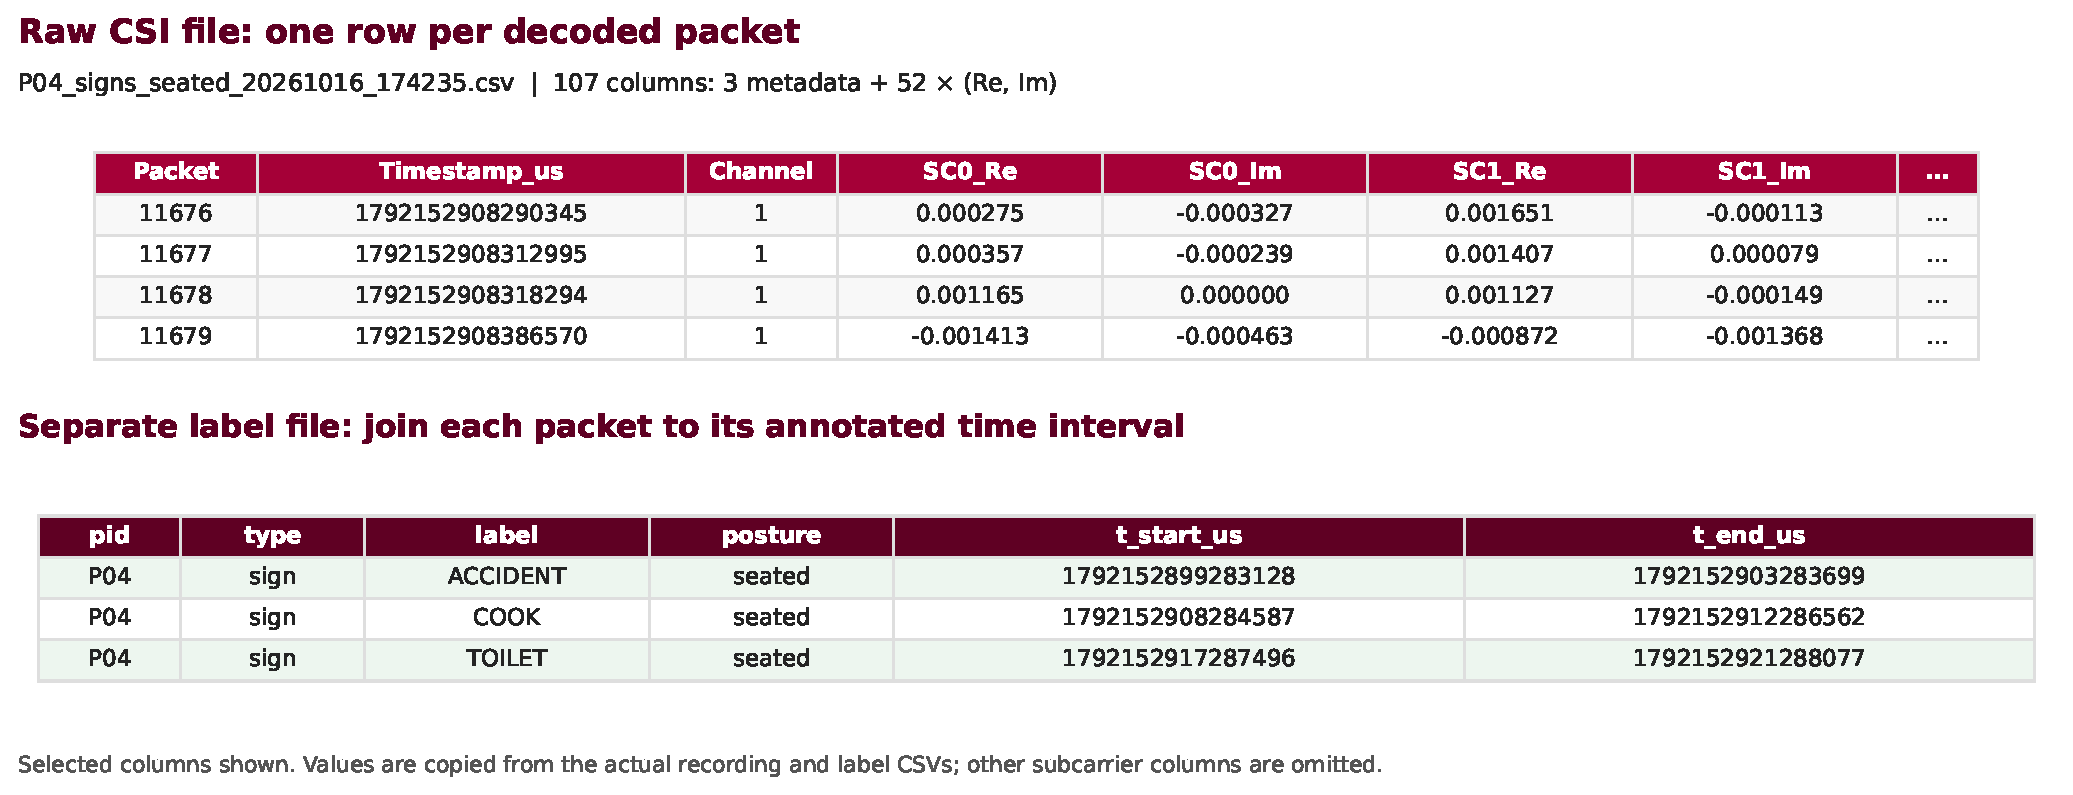
\includegraphics[width=0.97\linewidth,height=4.55cm,keepaspectratio]{current_impl/dataset_excerpt.pdf}
\end{center}
\vspace{-0.08cm}
\implnote{Actual CSV excerpt, selected columns. Raw rows contain packet/time/channel and complex CSI;
the separate label file supplies participant, type, label, posture and time boundaries.
Labels come from the collection cues/key presses; video alignment is not yet verified.}
\end{frame}
\begin{frame}{25. Current Dataset: Recording Rows per Class}
\roone
\begin{columns}[T,onlytextwidth]
\column{0.49\textwidth}
{\small\textbf{\color{AmritaMaroon}Actions}}\\[4pt]
\fontsize{7}{8.1}\selectfont\renewcommand{\arraystretch}{0.94}
\begin{tabular}{@{}lrr@{}}\toprule
\textbf{Class} & \textbf{Trials} & \textbf{Raw rows}\\\midrule
Answer phone & 67 & 46,741\\
Chop food & 40 & 25,679\\
Drink & 67 & 46,554\\
Eat & 67 & 46,401\\
Fall & 23 & 16,512\\
Light switch & 48 & 23,817\\
Pick up & 48 & 35,094\\
Sit--stand & 48 & 33,576\\
Stir pot & 40 & 25,174\\
TV remote & 67 & 39,134\\
Walk & 46 & 33,371\\
Wipe table & 67 & 44,783\\
\midrule\textbf{Total} & \textbf{628} & \textbf{416,836}\\
\bottomrule\end{tabular}
\column{0.49\textwidth}
{\small\textbf{\color{AmritaMaroon}Signs}}\\[4pt]
\fontsize{7}{8.1}\selectfont\renewcommand{\arraystretch}{0.94}
\begin{tabular}{@{}lrr@{}}\toprule
\textbf{Class} & \textbf{Trials} & \textbf{Raw rows}\\\midrule
ACCIDENT & 35 & 15,864\\
CALL & 35 & 15,815\\
COOK & 35 & 15,792\\
FAN & 35 & 15,956\\
HELLO & 35 & 16,019\\
HELP & 35 & 15,782\\
HOT & 35 & 16,097\\
HUNGRY & 35 & 16,140\\
LAMP & 35 & 15,689\\
PAIN & 35 & 16,051\\
TELEVISION & 35 & 15,641\\
THANKYOU & 35 & 15,697\\
TOILET & 35 & 15,875\\
WATER & 35 & 16,152\\
\midrule\textbf{Total} & \textbf{490} & \textbf{222,570}\\
\bottomrule\end{tabular}
\end{columns}
\vspace{0.10cm}
\implnote{Raw packets inside fully covered isolated label intervals; rest/ready and story steps excluded.
Partial P2 trials excluded. Chop/stir: P4/P5 only.}
\end{frame}
\begin{frame}{31. Current Model: Training and Evaluation}
\roone
\begin{center}
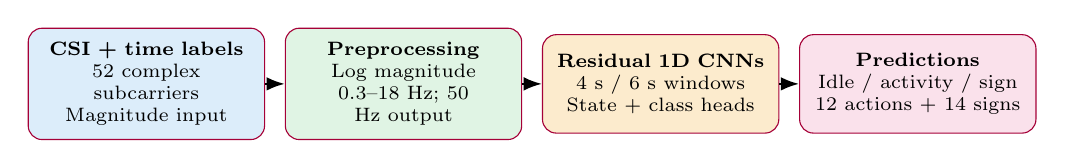
\begin{tikzpicture}[
 box/.style={draw=AmritaMaroon,rounded corners=5pt,align=center,minimum height=1.25cm,text width=2.65cm,font=\scriptsize,inner sep=5pt},
 arr/.style={-{Latex},thick}]
\node[box,fill=LightBlue] (raw) {\textbf{CSI + time labels}\\52 complex subcarriers\\Magnitude input};
\node[box,fill=LightGreen,right=0.25cm of raw] (prep) {\textbf{Preprocessing}\\Log magnitude\\0.3--18 Hz; 50 Hz output};
\node[box,fill=LightOrange,right=0.25cm of prep] (cnn) {\textbf{Residual 1D CNNs}\\4 s / 6 s windows\\State + class heads};
\node[box,fill=LightPink,right=0.25cm of cnn] (out) {\textbf{Predictions}\\Idle / activity / sign\\12 actions + 14 signs};
\draw[arr](raw)--(prep);\draw[arr](prep)--(cnn);\draw[arr](cnn)--(out);
\end{tikzpicture}
\end{center}
\vspace{0.12cm}
\begin{columns}[T,onlytextwidth]
\column{0.54\textwidth}
\footnotesize
\textbf{\color{AmritaMaroon}Five held-out-person tests}
\begin{itemize}\setlength{\itemsep}{3pt}
\item Initial fit: 3 people; validation: 1 other person.
\item Choose detector/action/sign roles on validation.
\item Refit selected networks on 4 people, two seeds.
\item Test only on the fifth person; repeat for all five.
\end{itemize}
\column{0.43\textwidth}
\footnotesize
\textbf{\color{AmritaMaroon}All-five deployment model}\\[5pt]
Two normalized four-second CNNs, one per seed, trained on all five people.\\[5pt]
Scales, masks and class order saved.\\[5pt]
Kaggle T4 $\times$2: \textbf{41.4 minutes}.
\end{columns}
\vspace{0.13cm}
\implnote{Scores come from held-out folds; the all-five refit has no independent score.
Inference is offline. ExtraTrees applies only to isolated action fusion (final weight: zero).}
\end{frame}
\begin{frame}{32. Current Results: Action Recognition}
\roone
{\footnotesize\textbf{\color{AmritaMaroon}311/628 correct (49.5\% accuracy)}
\hfill Mean held-out macro F1: \textbf{50.2\%}}
\begin{center}
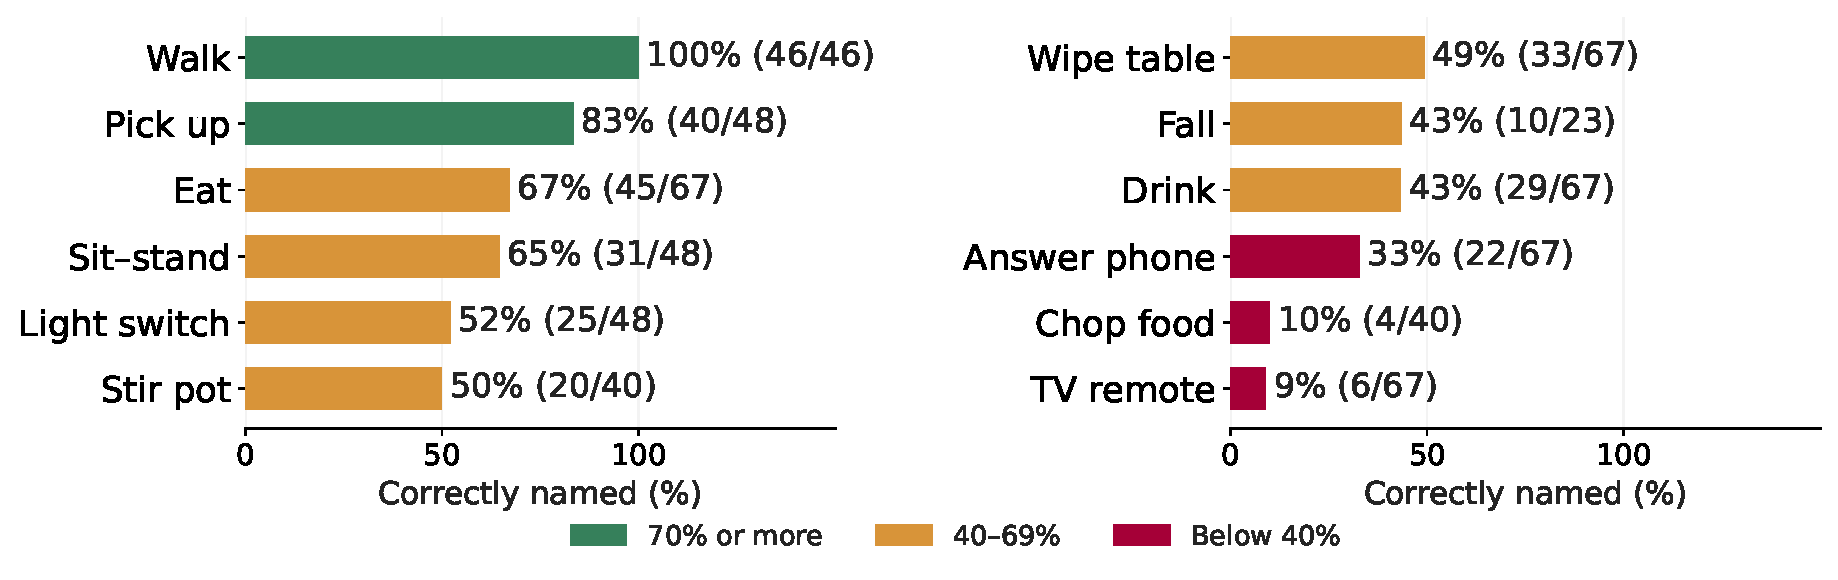
\includegraphics[width=\linewidth,height=4.45cm,keepaspectratio]{current_impl/action_class_performance.pdf}
\end{center}
\vspace{-0.08cm}
\implnote{P1--P5 isolated trials, known boundaries/type; bars show per-class recall.
\textbf{Strongest:} walk/pick up. \textbf{Weakest:} TV remote/chop/phone.
Chop/stir cover P4/P5 only.}
\end{frame}
\begin{frame}{33. Current Results: Sign Recognition}
\roone
{\footnotesize\textbf{\color{AmritaMaroon}171/490 correct (34.9\% accuracy)}
\hfill Mean held-out macro F1: \textbf{33.2\%}}
\begin{center}
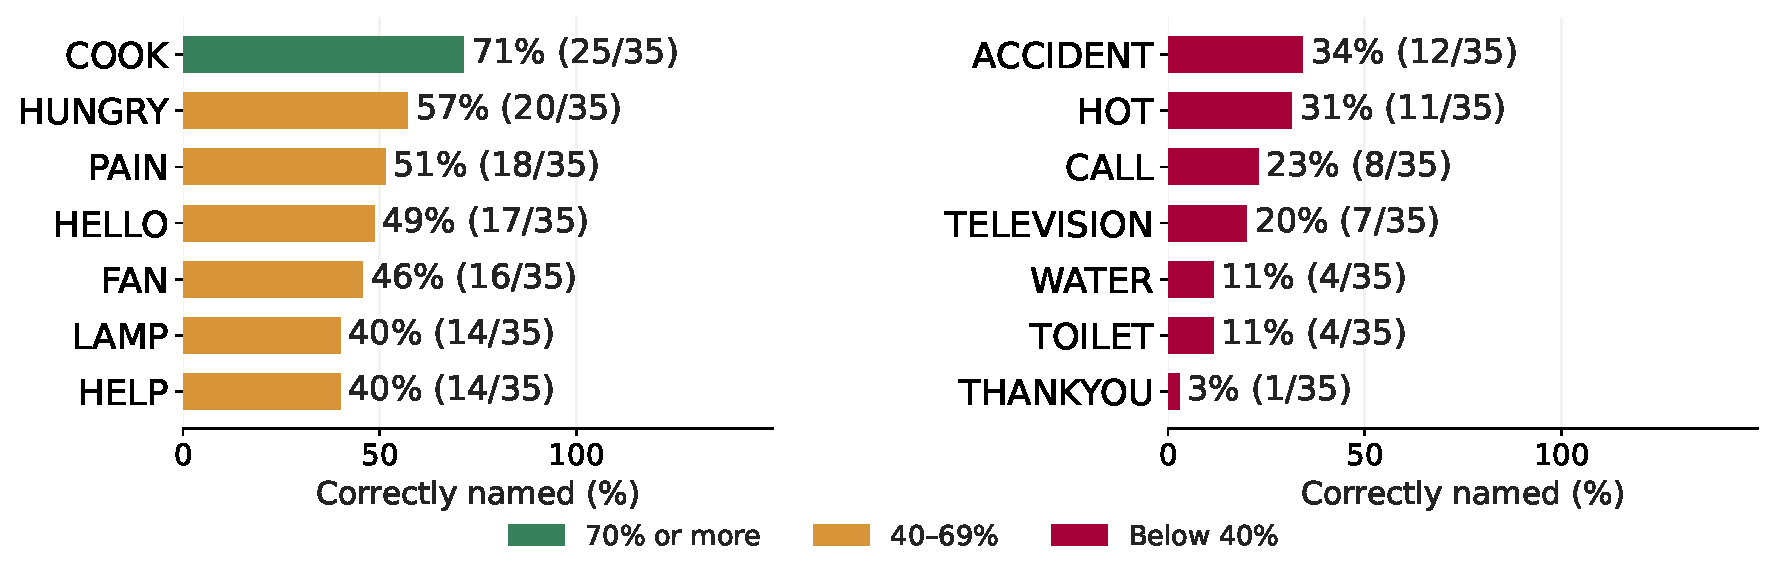
\includegraphics[width=\linewidth,height=4.45cm,keepaspectratio]{current_impl/sign_class_performance.pdf}
\end{center}
\vspace{-0.08cm}
\implnote{P1--P5: 350 standing + 140 seated trials; 35 per sign; known boundaries/type.
\textbf{Stronger:} COOK/HUNGRY/PAIN. \textbf{Weakest:} THANKYOU/WATER/TOILET.
Isolated seated signs cover P4/P5 only.}
\end{frame}
\begin{frame}{34. Current Results: Detection Threshold}
\roonefour
\begin{columns}[T,onlytextwidth]
\column{0.54\textwidth}
\footnotesize
\renewcommand{\arraystretch}{1.25}
\begin{tabular}{@{}lrr@{}}
\toprule
\textbf{Setting} & \textbf{Signs caught} & \textbf{False / hour}\\
\midrule
$\tau=0.3$: sensitive & 71.4\% & 27.5\\
$\tau=0.5$: middle & 68.9\% & 14.6\\
$\tau=0.7$: strict & 54.7\% & 10.5\\
\bottomrule
\end{tabular}
\vspace{0.25cm}

\footnotesize
Raise $\tau$ to reduce false triggers; fewer signs are caught.\\[5pt]
``Caught'' means detected, not correctly named.\\[5pt]
$\tau$ is a score cutoff, not calibrated certainty.
\column{0.43\textwidth}
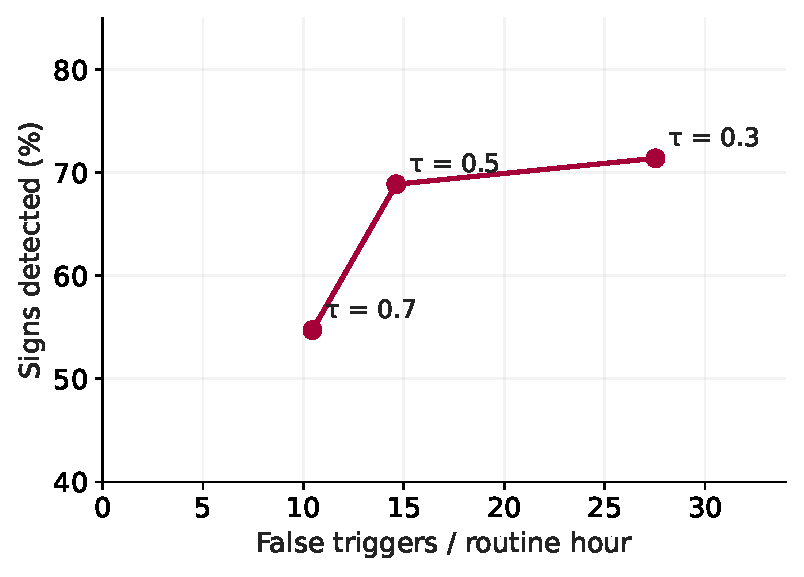
\includegraphics[width=\linewidth,height=4.25cm,keepaspectratio]{current_impl/threshold_tradeoff.pdf}
\end{columns}
\vspace{0.16cm}
\implnote{Fixed-threshold sweep: P1--P3, isolated + stories, 318 signs; mean over three people.
One-second smoothing/minimum run, one-second gap merge and $\pm$1 s matching.
Rates cover routine movement only (about 58 measured minutes), excluding idle/unknown periods.}
\end{frame}
\begin{frame}{35. Current Results: Continuous Story Recognition}
\roonefour
\begin{columns}[T,onlytextwidth]
\column{0.72\textwidth}
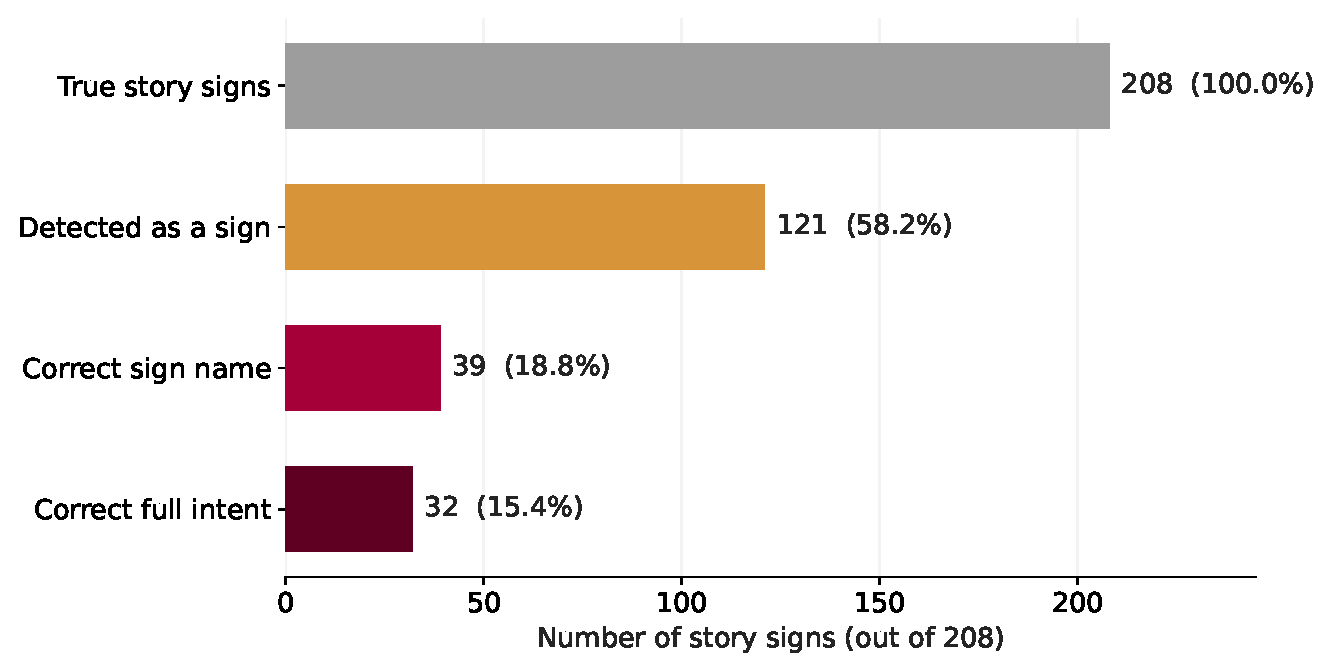
\includegraphics[width=\linewidth,height=4.55cm,keepaspectratio]{current_impl/story_recognition.pdf}
\column{0.25\textwidth}
\footnotesize
\textbf{\color{AmritaMaroon}Automatic story inference}\\[5pt]
No true sign boundaries or type are supplied.\\[6pt]
\textbf{58.2\%} of signs detected.\\[5pt]
\textbf{18.8\%} correctly named.\\[5pt]
\textbf{15.4\%} correct full intent.\\[7pt]
Continuous identity is the main remaining limitation.
\end{columns}
\vspace{0.13cm}
\implnote{All five people; validation-selected thresholds per fold; one-to-one IoU $\geq0.10$ matching.
This differs from the fixed-threshold sweep. There were 50 false triggers during 20.3 minutes of measured story routine activity.}
\end{frame}
\end{document}